\documentclass{article}
\usepackage{setspace}
\usepackage{listings}
\usepackage{color}
\usepackage{amsmath}
\usepackage{amssymb}
\usepackage{amsthm}
\usepackage{graphicx} 
\usepackage{float} 
\usepackage{fancyhdr}                                
\usepackage{lastpage}                                           
\usepackage{layout}   
\usepackage{subfigure} 
\definecolor{codegreen}{rgb}{0,0.6,0}
\definecolor{codegray}{rgb}{0.5,0.5,0.5}
\definecolor{codepurple}{rgb}{0.58,0,0.82}
\definecolor{backcolour}{rgb}{0.95,0.95,0.92}

\lstdefinestyle{mystyle}{
    backgroundcolor=\color{backcolour},   
    commentstyle=\color{codegreen},
    keywordstyle=\color{magenta},
    numberstyle=\tiny\color{codegray},
    stringstyle=\color{codepurple},
    basicstyle=\footnotesize,
    breakatwhitespace=false,         
    breaklines=true,                 
    captionpos=b,                    
    keepspaces=true,                 
    numbers=left,                    
    numbersep=5pt,                  
    showspaces=false,                
    showstringspaces=false,
    showtabs=false,                  
    tabsize=2
}
\pagestyle{fancy}  
\lhead{ZHANG HUAKANG}
\chead{Assignment 6} 
\rhead{DB92760} 
\renewcommand{\baselinestretch}{1.05}
\title{Assignment 6 of CISC 2002}
\author{ZHANG Huakang/DB92760}

\begin{document}
    \maketitle
    \section{}
        \paragraph{}
        \begin{equation*}
            \begin{split}
                \lim_{x\rightarrow 0}f(x)=&\lim_0^1 \frac{\sin x}{x}\\
                    =&\lim_0^1 \frac{\cos x}{1}\\
                    =&1\\
                    =&f(0)\\
            \end{split}
        \end{equation*}
        Thus, $f(x)$ is continuous on $[0,1]$
        \subsection{}
            \paragraph{}
            \begin{equation*}
                \begin{split}
                    I-h\approx&hf(\frac{h}{2})\\
                        =&1f(\frac{1}{2})\\
                        =&2\sin \frac{1}{2}\\
                        \approx&0.9589\\
                \end{split}
            \end{equation*}
        \subsection{}
            \paragraph{}
            \begin{equation*}
                \begin{split}
                    I_h\approx &\frac{h}{2}(f(0)+f(h))\\
                        =&\frac{1}{2}(1+sin 1)\\
                        \approx&0.9207\\
                \end{split}
            \end{equation*}
        \subsection{}
            \paragraph{}
            \begin{equation*}
                \begin{split}
                    I_h\approx&\frac{h}{6}(f(0)+4f(\frac{h}{2})+f(h))\\
                        =&\frac{1}{6}(1+4\times2\sin \frac{1}{2}+\sin 1)\\
                        \approx&0.9461\\
                \end{split}
            \end{equation*}
        \subsection{}
            \paragraph{}
            \begin{equation*}
                \begin{split}
                    h=&\frac{1-0}{6}\\
                        =&\frac{1}{6}\\
                \end{split}
            \end{equation*}
            \begin{equation*}
                \begin{split}
                    I_h\approx&\frac{h}{2}(f(x_0)+2(f(x_1)+f(x_2)+f(x_3)+f(x_4)+f(x_5))+f(x_6))\\
                        =&\frac{1}{12}(1+2(6\sin \frac{1}{6}+3\sin\frac{2}{6}+2\sin \frac{3}{6}+\frac{3}{2}\sin \frac{4}{6}+\frac{6}{5}\sin \frac{5}{6})+\sin 1)\\
                        \approx&0.9454
                \end{split}
            \end{equation*}
        \subsection{}
            \paragraph{}
            \begin{equation*}
                \begin{split}
                    I_h\approx&\frac{3}{h}(f(x_0)+4(f(x_1)+f(x_3)+f(x_5))+2(f(x_2)+f(x_4)))\\
                        \approx&0.9461
                \end{split}
            \end{equation*}
    \section{}
        \subsection{}
            \paragraph{}
            \begin{equation*}
                \begin{split}
                    I_h\approx&\frac{1}{3\times2^{n}}[f(x_0)+4\sum_{i=1}^{2^{n-1}}f(x_{2i-1})+2\sum_{i=1}^{2^{n-1}-1}f(x_{2i})+f(x_{2^n})]
                \end{split}
            \end{equation*}
            \lstinputlisting[language=Matlab,style=mystyle,caption=Code ]{code/Assignment_6_2_1.m}
            \lstinputlisting[language=Matlab,style=mystyle,caption=Output ]{code/Assignment_6_2_1_output}
            % \begin{equation*}
            %     \begin{split}
            %         r_1=&1.6768\\
            %         r_2=&0.9273\\
            %         r_3=&0.9983\\
            %         r_4=&0.9999\\
            %         r_5=&1.0000\\
            %         r_6=&1.0000\\
            %     \end{split}
            % \end{equation*}
        \subsection{}
            \begin{figure}[H] 
                \centering 
                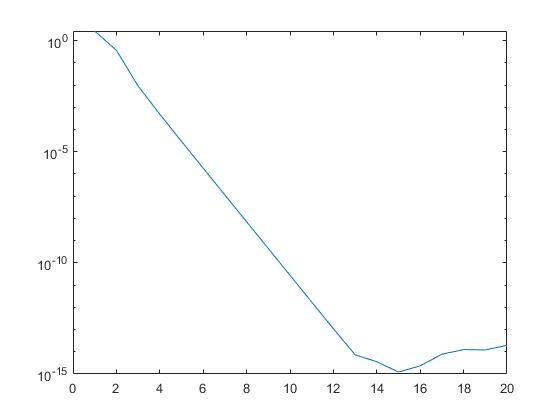
\includegraphics[width=0.9\textwidth]{img/Assignement_6_1.jpg}
                \caption{Figure} 
            \end{figure}

    \section{}
        \paragraph{}
        \begin{equation*}
            \begin{split}
                f(x)=&f(\frac{3h}{2})+f'(\frac{3h}{2})(x-\frac{3h}{2})+\frac{f''(\frac{3h}{2})}{2!}(x-\frac{3h}{2})^2\\
                    &+\frac{f^{(3)}(\frac{3h}{2})}{3!}(x-\frac{3h}{2})^3++\frac{f^{(4)}(\frac{3h}{2})}{4!}(x-\frac{3h}{2})^4\\
                    &+\frac{f^{(5)}(\frac{3h}{2})}{5!}(x-\frac{3h}{2})^5+r_5(x-\frac{3h}{2})^5+...\\
            \end{split}
        \end{equation*}

        \begin{equation*}
            \begin{split}
                \int_0^{3h}f(x)dx=&3hf(\frac{3h}{2})+\frac{9}{4}h^3\frac{f''(\frac{3h}{2})}{2!}+\frac{243}{80}h^5\frac{f^{(4)}(\frac{3h}{2})}{4!}+...\\
                e=&\int_0^{3h}f(x)dx-\frac{3h}{8}(f(0)+3f(h)+3f(2h)+f(3h))
            \end{split}
        \end{equation*}
                \begin{equation*}
            \begin{split}
                f(0)=&f(\frac{3h}{2})-\frac{3h}{2}f'(\frac{3h}{2})+\frac{3h}{2} ^2\frac{f^{''}(\frac{3h}{2})}{2!}-\frac{3h}{2} ^3\frac{f^{(3)}(\frac{3h}{2})}{3!}+...\\
                f(h)=&f(\frac{3h}{2})-\frac{h}{2}f'(\frac{3h}{2})+\frac{h}{2} ^2\frac{f^{''}(\frac{h}{2})}{2!}-\frac{h}{2} ^3\frac{f^{(3)}(\frac{3h}{2})}{3!}+...\\
                f(2h)=&f(\frac{3h}{2})+\frac{h}{2}f'(\frac{3h}{2})+\frac{h}{2} ^2\frac{f^{''}(\frac{h}{2})}{2!}+\frac{h}{2} ^3\frac{f^{(3)}(\frac{3h}{2})}{3!}+...\\
                f(3h)=&f(\frac{3h}{2})+\frac{3h}{2}f'(\frac{3h}{2})+\frac{3h}{2} ^2\frac{f^{''}(\frac{3h}{2})}{2!}+\frac{3h}{2} ^3\frac{f^{(3)}(\frac{3h}{2})}{3!}+...\\
            \end{split}
        \end{equation*}
        \begin{equation*}
            \begin{split}
                e=&-\frac{9}{10}h^5\frac{f^{(4)}(\frac{3h}{2})}{4!}\\
                    =&O(h^5)
            \end{split}
        \end{equation*}
    \section{}
        \subsection{}
            \paragraph{}
            \lstinputlisting[language=Matlab,style=mystyle,caption=Code ]{code/Assignment_6_4_1.m}
            \begin{figure}[H] 
                \centering 
                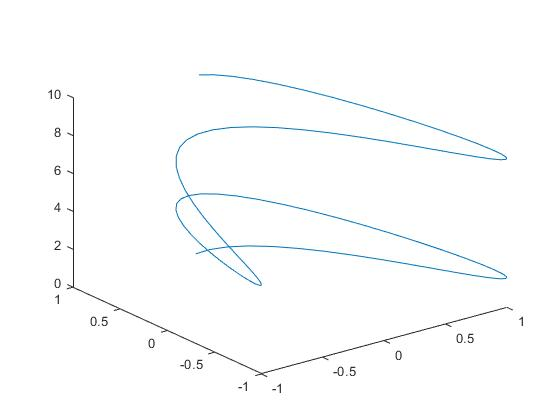
\includegraphics[width=0.9\textwidth]{img/Assignement_6_2.jpg}
                \caption{Figure} 
            \end{figure}
        \subsection{}
            \paragraph{}
            \begin{equation*}
                \begin{split}
                    s=&\int_0^{3\pi}\sqrt{(\frac{dx}{dt})^2+(\frac{dy}{dt})^2+(\frac{dz}{dt})^2}dt\\
                        =&\int_0^{3\pi}\sqrt{\cos^2 t+4\sin^2 2t+1}dt\\
                \end{split}
            \end{equation*}
            $$h=\frac{3\pi}{14}$$
            \begin{equation*}
                \begin{split}
                    s=&\frac{h}{3}(f_0+4f_1+2f_2...4f_{14}+f_{15})\\
                \end{split}
            \end{equation*}
            \lstinputlisting[language=Matlab,style=mystyle,caption=Code ]{code/Assignment_6_4_2.m}
            \lstinputlisting[language=Matlab,style=mystyle,caption=Output ]{code/Assignment_6_4_1output}
        \subsection{}
            \lstinputlisting[language=Matlab,style=mystyle,caption=Code ]{code/Assignment_6_4_3.m}
            \lstinputlisting[language=Matlab,style=mystyle,caption=Output ]{code/Assignment_6_4_3output}
    \section{}
        \subsection{}
            \paragraph{}
            \lstinputlisting[language=Matlab,style=mystyle,caption=Code ]{code/Assignment_6_5_1.m}
            \begin{figure}[H] 
                \centering 
                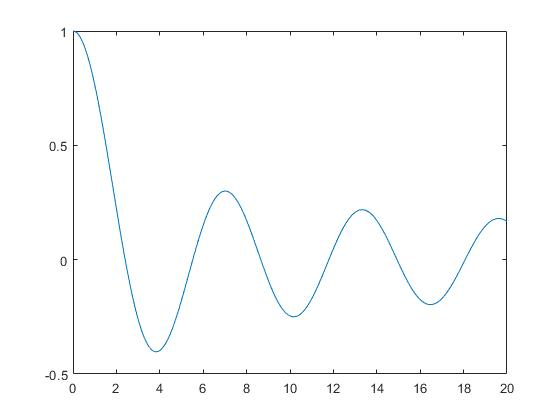
\includegraphics[width=0.9\textwidth]{img/Assignement_6_3.jpg}
                \caption{Figure} 
            \end{figure}
        \subsection{}
            \lstinputlisting[language=Matlab,style=mystyle,caption=Output ]{code/Assignment_6_5_1output}
        \subsection{}
            \lstinputlisting[language=Matlab,style=mystyle,caption=Code ]{code/Assignment_6_5_2.m}
            \lstinputlisting[language=Matlab,style=mystyle,caption=Output ]{code/Assignment_6_5_2}
\end{document}
